\documentclass{standalone}
\usepackage{tikz}
\usepackage{pgfplots}
\pgfplotsset{compat=newest}
\usepackage{amsmath}
\usepackage[american]{circuitikz}
\usepackage{cmbright}

\definecolor{myred}{RGB}{170,0,0}
\definecolor{myblue}{RGB}{0,0,220}
\definecolor{mygreen}{RGB}{0,150,0}
\definecolor{myorange}{RGB}{255,127,0}
\definecolor{mybrown}{RGB}{150,75,0}

\begin{document}
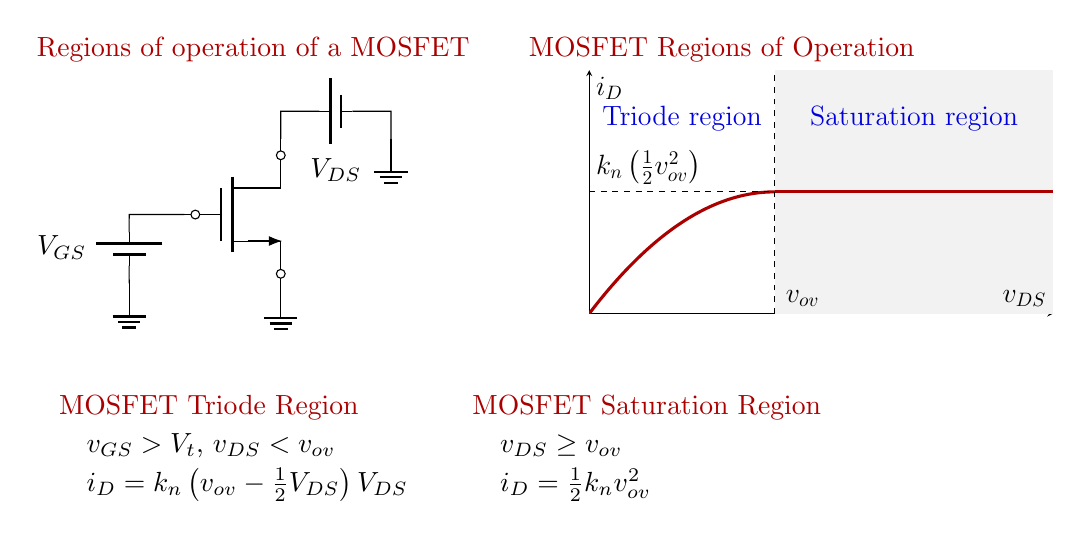
\begin{tikzpicture}
    \begin{scope}[scale=0.7]
        % Title
        \node[anchor=center, color=myred] at (-0.5, 2.5) {Regions of operation of a MOSFET};
        
        % npn BJT sumbol
        \draw (0, -0.5) node[nmos, scale=1.25] (Q) {};
        \draw (Q.gate) 
            to ++(-1, 0)
            to[battery1, l_=$V_{GS}$] ++(0, -1.25)
            node[ground] {};
        \draw (Q.source)
            to ++(0, 0.1)
            node[ground] {};
        \draw (Q.drain)
            to ++(0, 0.5)
            to[battery1, l_=$V_{DS}$] ++(2.0, 0)
            to ++(0, -0.5)
            node[ground] {};
        \draw[-Latex, thin] ($(Q.source) + (-0.6, 0.895)$) -- ++(0.625, 0);
        % Add the transistor nodes.
        \node[ocirc] at ($(Q.gate) + (0.2, 0)$) {};
        \node[ocirc] at ($(Q.source) + (0, 0.3)$) {};
        \node[ocirc] at ($(Q.drain) + (0, -0.3)$) {};
    \end{scope}

    \begin{scope}[scale=0.7, xshift=6.0cm]
        \node[anchor=center, color=myred] at (2, 2.5) {MOSFET Regions of Operation};
        \begin{axis}[
            at={(-6.0, -65)},
            anchor=origin,
            width=10cm,
            height=6cm,
            xmin=0, xmax=1.25,
            ymin=0, ymax=1.25,
            samples=200,
            axis lines=center,
            xlabel={\Large $v_{DS}$},
            ylabel={\Large $i_D$},
            xtick=\empty,
            ytick=\empty,
            clip=true,
        ]
        % Parametric forward bias: V = x, I = f(V)
        % v_GS1
        \draw[fill=gray!10, draw=none] (0.5, 0) rectangle (1.25, 1.25);
        \addplot[myred, ultra thick, domain=0:0.5] (x, {5 * (0.5 * x - 0.5 * x * x)});
        \addplot[myred, ultra thick, domain=0.5:1.25] (x, {0.625});
        \draw [black, dashed, thin] (0., 0.625) -- (0.5, 0.625);
        \draw [black, dashed, thin] (0.5, 0) -- (0.5, 1.25);
        \node [anchor=south, color=black] at (0.575, 0) {\Large $v_{ov}$};
        \node [anchor=west, color=black] at (0.0, 0.75) {\Large $ k_n \left(\frac{1}{2}v_{ov}^2\right)$};
        \node[anchor=center, color=myblue] at (0.25, 1.0) {\Large Triode region};
        \node[anchor=center, color=myblue] at (0.875, 1.0) {\Large Saturation region};
        \end{axis}
    \end{scope}

    \begin{scope}[scale=0.7, xshift=-1.7cm, yshift=-4.0cm]
        % Triode region
        \node[anchor=west, color=myred] at (-2.5, 0) {MOSFET Triode Region};
        \node[anchor=west, color=black] at (-2.0, -0.7) {$v_{GS} > V_t$, $v_{DS} < v_{ov}$};
        \node[anchor=west, color=black] at (-2.0, -1.4) {$i_{D} = k_n\left(v_{ov} - \frac{1}{2}V_{DS}\right)V_{DS}$};
        % Saturation region
        \node[anchor=west, color=myred] at (5, 0) {MOSFET Saturation Region};
        \node[anchor=west, color=black] at (5.5, -0.7) {$v_{DS} \geq v_{ov}$};
        \node[anchor=west, color=black] at (5.5, -1.4) {$i_{D} = \frac{1}{2}k_nv_{ov}^2$};
    \end{scope}
\end{tikzpicture}
\end{document}